\section{Overview}
\label{sec:methodOverview}
Figure \ref{fig:methodOverview} summarizes our procedure for quantifying the disagreement between different saliency explanation methods. Initially, we train each targeted black box on the selected dataset that consists of x-ray images and matching masks. The specifics of this dataset will be discussed in depth in chapter \ref{ch:experimentsAndResult}. Subsequently, we apply the attribution algorithm of the chosen explanation methods to the test set, which generates an explanation for the black box per each test example. We then calculate the level of disagreement by using disagreement metrics for each pair of explanations per test example and aggregate the outcomes to create a comparison heatmap. Finally, we examine the heatmaps to determine whether there is any significant disagreement.

\begin{figure}
    \centering
    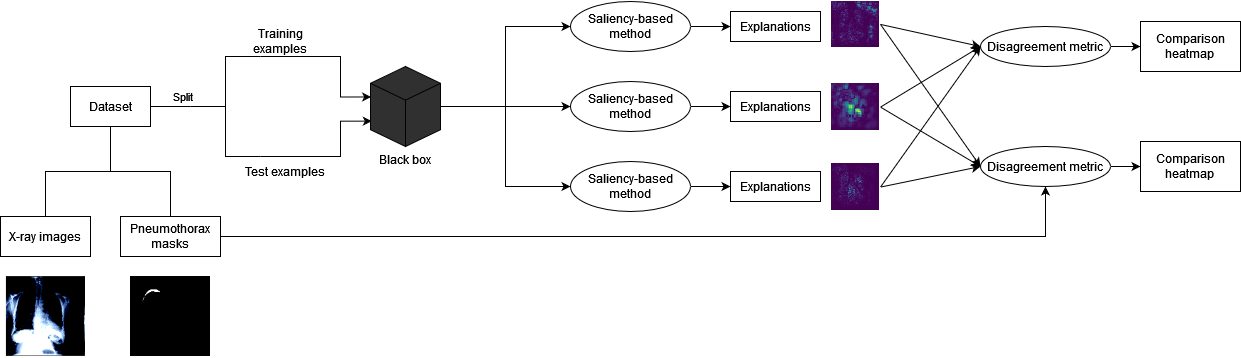
\includegraphics[width=\textwidth]{images/method-overview.png}
    \caption{An overview of the steps we've taken to quantify the disagreement between the explanation methods. These steps are applied per black box.}
    \label{fig:methodOverview}
\end{figure}

Note that this procedure is applied per black box. In our experiments in chapter \ref{ch:experimentsAndResult}, we applied this procedure to two different black boxes and analyzed the outcomes for both of them.